\label{sec:ouu_overview}

The FOQUS OUU module supports several variants of optimization under 
uncertainty. This chapter first presents the mathematical formulations 
of these variants. Subsequently, details of the OUU graphical user 
interface will be discussed.

\section{OUU Variables}

Suppose a simulation model is available for an OUU study. Let this 
simulation model be represented by the following function:
\begin{equation}
Y = F(Z_1,Z_2,Z_3,Z_4),
\end{equation}
which is characterized by four types of variables:
\begin{enumerate}
\item {\textbf{Design/Decision/Optimization variables}
\begin{itemize}
\item{Notation: $Z_1$ with dimension $n_1$}
\item{Definition: Design variables are continuous variables
that may be bounded or unbounded. They are generally the
set of optimization variables in a single-stage optimization
or the set of outer optimization variables in the two-stage
optimization.}
\end{itemize}
}

\item{\textbf{Recourse/Operating variables}
\begin{itemize}
\item{Notation: $Z_2$ with dimension $n_2$} 
\item{Definition: Operating
variables are optimization variables in the inner
optimization for a given scenario (or realization)
of the uncertain variables in a two-stage optimization.}
\end{itemize}
}

\item{\textbf{Discrete uncertain variables}
\begin{itemize}
\item{Notation: $Z_3$ with dimension $n_3$}
\item{Definition: Discrete variables are uncertain
variables that have an enumerable set of states
(called scenarios) such that each state is associated 
with a finite probability and the sum of probabilities
for all the scenarios is equal to $1$.}
\end{itemize}
}

\item{\textbf{Continuous uncertain variables}
\begin{itemize}
\item{Notation: $Z_4$ with dimension $n_4$}
\item{Definition: Continuous uncertain variables are
associated with a joint probability distribution
function from which a sample can be drawn to compute
the basic statistics.}
\end{itemize}
}
\end{enumerate}

\section{OUU Objective Functions}

In the presence of uncertainties, OUU seeks to find the
optimal solution in some statistical sense. For example,
an optimization goal may to be find the design settings
that minimizes the statistical mean of the system
response. Other popular objective functions are:
\begin{enumerate}
\item a linear combination of statistical mean and
      standard deviation of some selected output,
\item probability of exceeding the best value is smaller
      than some percentage at any point in the design
      space (this is analogous to conditional value at
      risk).
\end{enumerate}
Note that these metrics are defined in the design variable 
space - that is, at each iteration of an OUU algorithm, the
selected metric will be computed for the decision point
under consideration. Since the calculation of these
statistical metrics requires a sample (possibly large),
OUU can benefit from parallel computing capabilities
(e.g., the Turbine gateway).

\section{Mathematical Formulations}

FOQUS supports two types of OUU methods: single-stage
OUU and two-stage OUU. The main difference between
single-stage and two-stage OUU is the presence of the
recourse (or operational) variables.  Strictly speaking,
since recourse variables are generally hidden (they are
only needed in the inner stage and their values are not
used in the outer stage of two-stage OUU), the distinction
between single-stage and two-stage OUU is not clear.
Nevertheless, for the sake of clarify, we will describe
details of each formulation separately. The current
OUU does not support linearly or nonlinearly-constrained
optimization.

\subsection{Single-Stage Formulation}

In this formulation, there is no recourse variable: 
\begin{equation}
Y = F(Z_1, Z_3, Z_4)
\end{equation}
and the optimization problem becomes:

\begin{equation}
\min_{Z_1} \mathbf{\Phi}_{Z_3,Z_4} 
\left[ F(Z_1,Z_3,Z_4)
\right]
\end{equation}
where
$\Phi_{Z_3,Z_4} [F(Z_1,Z_3,Z_4)]$ is the statistical
metric (one of the three options given above).

For example, if the objective function is the statistical
mean, then the formulation becomes:
%\[
\begin{equation}
\min_{Z_1} \mathbf{E}_{Z_3,Z_4} [F(Z_1,Z_3,Z_4)]  
\approx 
\min_{Z_1} {
\sum^{n_3}_{j=1} \pi_j \left( 
\int {F(Z_1,Z_3,Z_4)  
P(Z_4) d Z_4} \right)}
\end{equation}
%\]
where, again, $n_3$ is the number of scenarios
for the discrete uncertain variables, $\pi_j$ is the
probability of the $j$-th scenario, and $P(Z_4)$ is the 
joint probability of the continuous uncertain variables.

\subsection{Two-Stage Formulation}

In this formulation all four types of variables are present.
The objective function is given by:
\begin{equation}
%\[
\begin{array}{lcl}
& & \displaystyle \min_{Z_3,Z_4}
\mathbf{\Phi}_{Z_3,Z_4} \left[
\min_{Z_2} 
F(Z_1,Z_2,Z_3,Z_4) \right]. 
\end{array}
%\]
\end{equation}
If the objective function is the statistical mean, the
formulation becomes:
%\[
\begin{equation}
\begin{array}{lcl}
& & \displaystyle \min_{Z_1}
\mathbf{E}_{Z_3,Z_4} \left[
\min_{Z_2} F(Z_1,Z_2,Z_3,Z_4) \right]\\ 
&\approx& \displaystyle \min_{Z_1} \sum^{n_3}_{j=1} \pi_j 
\left( 
\int \left[
\min_{Z_2} F(Z_1,Z_2,Z_3,Z_4) \right] P(Z_4) d Z_4
\right)
\end{array}
\end{equation}
%\]
Let
\begin{equation}
G(\mathbf{Z_1,Z_3,Z_4}) = \min_{Z_2} F(Z_1,Z_2,Z_3,Z_4).
\end{equation}
Then the two-stage equation can be rewritten as:
\begin{equation}
%\[
\begin{array}{lcl}
& & \displaystyle \min_{Z_1}
\mathbf{E}_{Z_3,Z_4} \left[
G(Z_1,Z_3,Z_4) \right]\\ 
&\approx& \displaystyle \min_{Z_1} \sum^{n_3}_{j=1} \pi_j 
\left( \int 
G(Z_1,Z_3,Z_4) P(Z_4) d Z_4
\right)
\end{array}
%\]
\end{equation}
which is a single-stage OUU with respect to the $G$ function.

\section{OUU User Interface}

The OUU module enables the user to perform optimization under uncertainty studies 
on a flowsheet. From the OUU tab, the user can set up the different types of
optimization parameters, select from the different OUU options, and run the 
optimization. This screen is shown in Figure \ref{fig:ouu_screen}.

%%% INSERT: OUU Screen
\begin{figure}[H]
\centering 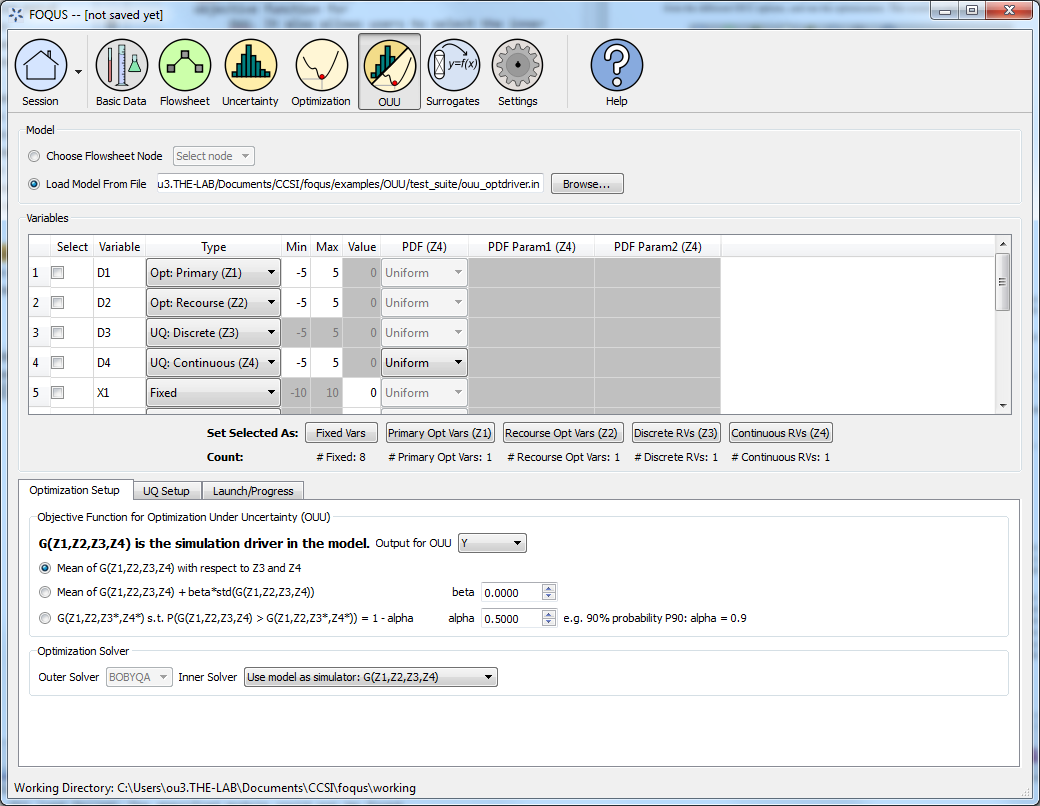
\includegraphics[width=6.5in,height=4in,keepaspectratio]{Chapt_ouu/figs/1_OUUScreen}
\caption{Optimization Under Uncertainty Screen}
\label{fig:ouu_screen}
\end{figure}

\begin{enumerate}
\item
	\bu{Model} provides two options for setting up the model: (1) select a node from
         the flowsheet that has already been instantiated; or (2) load the model from 
         a file in the PSUADE full file format (with the {\sf opt\_driver} variable
         set to the simulation executable.)
\item 
	\bu{Variables} displays all variables defined in the model that can be used in
         this context. Each available variable can be set to either one of
         the 5 types:
         \begin{itemize}
         \item fixed (the parameter's value is fixed throughout the optimization
         process)
         \item primary (parameter for the outer optimization)
         \item recourse (parameter for the
         inner optimization)
         \item discrete (categorical uncertain parameter that contributes to
         scenarios)
         \item continuous (continuous uncertain parameter with a given
         probability distribution)
         \end{itemize} 
\item
	\bu{Optimization Setup} allows users to select the objective function for 
         OUU. It also allows users to select the inner optimization solver. There
         are two options for the inner solver: (1) the simulation model provided 
         by users is an optimizer itself, and (2) the simulation provided by 
         users needs to be wrapped around by another optimizer in FOQUS.

\item
	\bu{UQ Setup} allows users to set up the continuous uncertain parameters.
        There are two options: (1) FOQUS can generate a sample internally, or (2)
        a user-generated sample can be loaded into FOQUS.  The sample size should
        be larger than the number of continuous uncertain parameters. Optionally,
        response surface can be turned on to enable the statistical moments to be
        computed more accurately even with small samples. Users can also select
        a smaller subset of the sample for building response surfaces and evaluate
        the response surfaces with the larger samples.

\item
	\bu{Launch/Progress} has the `Run OUU' button to launch OUU runs.
\end{enumerate}

